% Activate the following line by filling in the right side. If for example the name of the root file is Main.tex, write
% "...root = Main.tex" if the chapter file is in the same directory, and "...root = ../Main.tex" if the chapter is in a subdirectory.
 
%!TEX root =  

\chapter{Documentation}\label{doc}

\minitoc

This chapter provides documentation for the Privacy Advisor system. It gives an overview over the available source code documentation (JavaDoc), instructions for how to compile and install the system, and how it is used via. its GUI and command line interfaces.

\section{Source Code Documentation} 

The source code is documented using JavaDoc which is a tool that generates documentation in HTML format based on source code comments in Java, and is a standard part of the Java SDK. The JavaDoc for the Privacy Advisor system follows Sun Microsystems' style guide for writing JavaDoc comments\footnote{See: http://www.oracle.com/technetwork/java/javase/documentation/index-137868.html}. 

Source code documentation plays an important role in this project, as it is an early software prototype to be used in research which means that the code is then likely to be modified. The aim of the source code documentation is to supplement UML design documents to facilitate future development.



\section{Installation}


\subsection{Compilation in Eclipse} \label{LocalInst}
The simplest way to make the program run as a stand-alone program on a Java Virtual Machine is to compile the source code to a runnable jar file. This section covers how this is done in the Eclipse environment.

\subsubsection{Open Export Wizard}
This can be done by right clicking the project in Eclipse, choosing \texttt{Export}, type in \texttt{jar} in the new window that opens up and choose \textbf{Runnable Jar File}, before clicking \textbf{Next}. These steps are shown in the two figures \ref{exportFirstStep} and \ref{exportSecondStep}.

\begin{wrapfigure}{r}{0.4\textwidth}
  \vspace{-10pt}
  \begin{centering}
    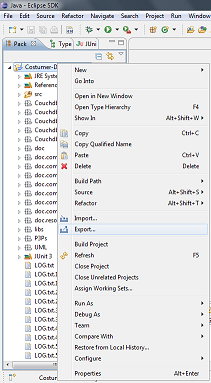
\includegraphics[width = .38\textwidth]{Documentation/export.png}
    \vspace{-10pt}
    \caption{First step: right click and choose "export".}
    \vspace{-10pt}
    \label{exportFirstStep}
    \end{centering}
  \end{wrapfigure}

  \subsubsection{Select GUI or CLI}
  The next step is to select which class file is to be the main class\footnote{Privacy Advisor has two files containing a main method. One is for running the CLI version, one for the GUI version.}; in the \textbf{Launch configuration} dropdown select either \texttt{PrivacyAdvisor} or \texttt{PrivacyAdvisorGUI}.

\texttt{PrivacyAdvisor} is selected to compile the command line version, and the \texttt{PrivacyAdvisorGUI} is selected for command line. Then choose the export destination, and choose \texttt{Package requires libraries into generated JAR} as the library handling. Pressing finish to start exporting the program. These steps are shown in figure \ref{exportLastStep}.


  \begin{wrapfigure}{l}{0.5\textwidth}
    \begin{centering}
      \vspace{-10pt}
      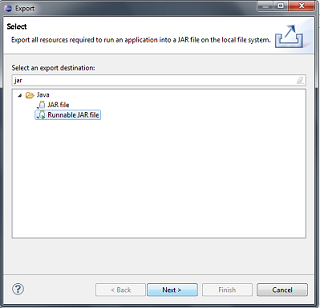
\includegraphics[width = .48\textwidth]{Documentation/export_jar.png}
      \vspace{-10pt}
      \caption{Second step: choose runnable jar.}
      \vspace{-10pt}
      \label{exportSecondStep}
    \end{centering}
  \end{wrapfigure}

\subsubsection{Configuration File}
Before running the program PrivacyAdviser.cfg has to be put in the same folder as the exported jar file. If the database file and the weights file at the same folder, their location have to be specified in the PrivacyAdviser.cfg file. 

\begin{wrapfigure}{l}{0.5\textwidth}
  \begin{centering}
    \vspace{-10pt}
    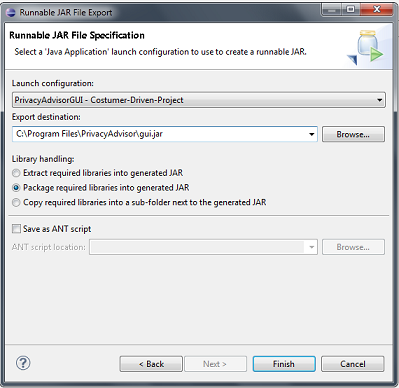
\includegraphics[width = .48\textwidth]{Documentation/export_last.png}
    \vspace{-10pt}
    \caption{Third step: choose launch config, destination and library handling.}
    \vspace{-10pt}
    \label{exportLastStep}
  \end{centering}
\end{wrapfigure}


\subsubsection{Sample Run}
To run the program, navigate to the folder where the jar file is stored and type the following command:

\framebox[1.1\width]{\texttt{java -jar filename.jar}}

Now the program should start (even if it's the cli or gui version). This is shown in figure \ref{runProgram}.

\begin{figure}
  \begin{centering}
    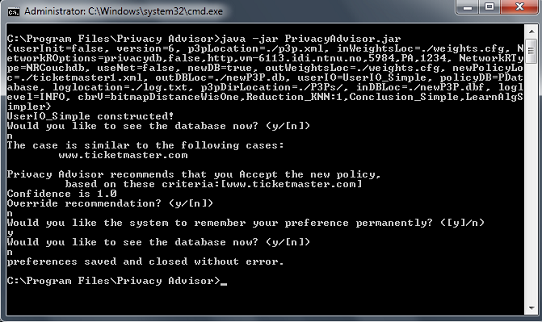
\includegraphics{Documentation/cli.png}
    \caption{Running the program.}
    \label{runProgram}
  \end{centering}
\end{figure}


\subsection{Server Installation}
The CouchDB server is a default Ubuntu installation on a VMware virtual machine provided by NTNU IDI, with CouchDB installed using the command:

\framebox[1.1\width]{\texttt{sudo apt-get install couchdb}}

The database server was configured via \emph{futon} (the default web interface, located at \texttt{localhost:5984\/\_util}) to provide a database entitled \texttt{privacydb}, with a non-administration user (details noted in default program configuration file).

\section{User Interfaces}
The Privacy Adviser consists, as mentioned in section \ref{LocalInst}, of two different user interfaces. The advantage of the GUI is that it's easier to see the contents in the database before and after the program runs. The command line interface better suited for repetitive tasks, in particular for batch type testing. The command line interface operates according to the options given when starting the program, either as command line parameters or through the configuration file. This is explained in detail in section \ref{cliExplained}.

\subsection{Command Line Interface} \label{cliExplained}
By running the program from the command line options can be set directly as command line parameters when starting the program. If no parameters are given, the options set in the PrivacyAdviser.cfg will be used. Options added as command line parameters have priority over configuration file options.

As an example consider the location of the database. By default, the options in PrivacyAdviser.cfg is set to replace the old database with the new database when the program exits. If the user wants to store the changes to a new database file, the \texttt{outDBLoc} parameter needs to be set to a new file.

There are two ways to change this. The first is to set the \texttt{outDBLoc} parameter at the command line. This will override the config file for this particular run. 

\framebox[1.1\width]{\texttt{java -jar privacyAdvisor.jar -outDBLoc newDatabase.db}}

More options can be added in this manner, and for the options that are not specified, the default options in the config file will be used. For a complete list of the options see table \ref{configTable}.

The second approach is to change the outDBLoc in the configuration file directly.

\subsection{Graphical User Interface}
When using the graphical user interface, the left hand pane gives an overview of the all the policies and cases in the database as a tree-structure. The right hand pane gives a similar view of how the new policy. This can be seen in figure \ref{guiFigure}. The GUI is started from the command line the same way the CLI is started.

\subsubsection{Obtaining Advice for a Policy}
When the GUI is stared, it automatically loads the database file, and displays the tree-structure. Pressing the \texttt{Run} button in the \texttt{Privacy Advisor} menu runs the CBR classifier and displays a message box containing an advice along with a measure of confidence and references to the sites on which the decision is based.

%%% TODO: edited hitherto

If we want to change the location of the database, the new policy or anything else we can press the \texttt{Configuration} button and make the changes in the \texttt{Configuration Editor} window that shows up. This Configuration Editor window is showed in figure\ref{guiConfig}.

 \begin{wrapfigure}{r}{0.5\textwidth}
     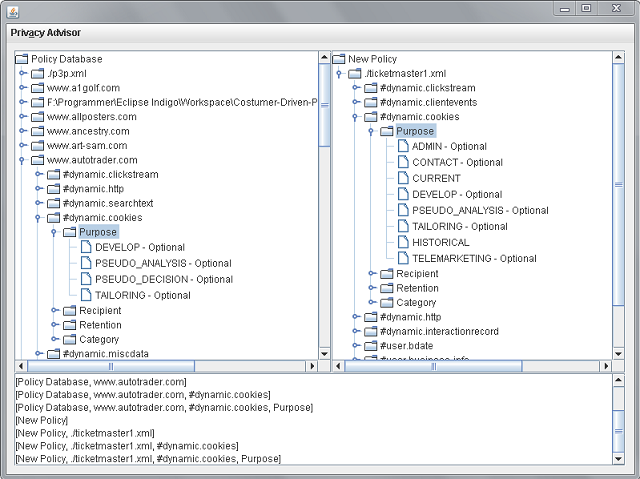
\includegraphics[width = .48\textwidth]{Documentation/gui.png}
     \caption{The GUI.}
   \label{guiFigure}
 \end{wrapfigure}

   \begin{wrapfigure}{r}{0.5\textwidth}
     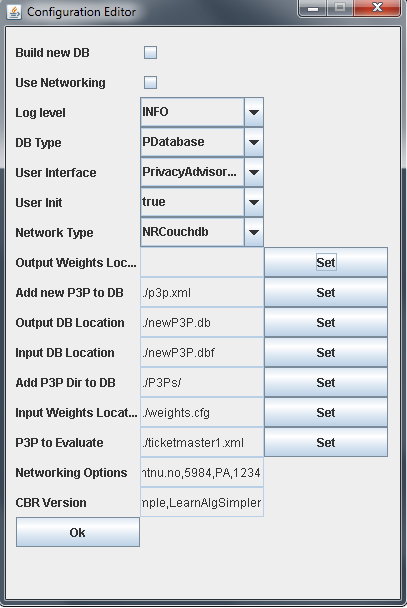
\includegraphics[width = .48\textwidth]{Documentation/gui_config.png}
     \caption{The GUI.}
   \label{guiFigure}
 \end{wrapfigure}


\subsubsection{Configuration Files}

Table~\ref{configTable} gives an overview over the configuration file parameters.

\begin{center}
  \begin{table}[h!]
    \label{configTable}
    \begin{tabular} { | l | l | p{7cm} | }
      \hline
      \textbf{Item} & \textbf{Datatype} & \textbf{Description} \\ \hline
      loglocation & string/filepath  & where the log is written to. can't be changed once the UI is  called. \\ \hline
      loglevel & string/logging level	& what level to log at. \\ \hline
      inDBLoc & string/filepath	& where to read the past history from. \\ \hline
      outDBLoc & string/filepath & where to write DB- defaults to where it reads from. \\ \hline
      inWeightsLoc& string/filepath & where to read the weights config file from. \\ \hline
      outWeightsLoc	& string/filepath & where to write DB- defaults to where it reads from. \\ \hline
      newDB & string/boolean & are we overwriting/ignoring an old database. \\ \hline
      p3pLocation & string/filepath & a p3p to be added to the history. \\ \hline
      p3pDirLocation	& string/FOLDERpath& a folder of p3ps to be added to the history. \\ \hline
      blanketAccept & string/boolean & accept the advisers recommendation. \\ \hline
      newPolicyLoc & string/filepath	& the new policy to be parsed. \\ \hline
      userInit & string/boolean	& true if some initialization occurs via the user interface. \\ \hline
      userResponse & string/action	& the response to the suggestion, if know beforehand. \\ \hline
      cbrV & string/CBR & parses for algorithms, etc to use. See CBR:parse(String). \\ \hline
      userIO & string/UIO	& the user interface to use. see Gio:selectUI. \\ \hline
      policyDB & string/policyDB & select the database type. see Gio:selectPDB . \\ \hline
      genConfig	& string/filepath & load an alternate configuration file. \\ \hline
      networkRType & string/classname & the name of a networkR class. \\ \hline
      networkROptions & string/commasepoptions	& the options necessary for the above networkR class. \\ \hline
      confidenceLevel & string/double & the confidence level at which the algorithm trusts itself; if below this, it uses the server's suggestion. \\ \hline
      useNet & string/boolean & whether to activate network functionality. \\ \hline
      \hline
    \end{tabular}
    \caption{Configuration file parameters.}
  \end{table}
\end{center}

\subsubsection{Building a Database}

\textbf{CLI}: To build a new database from a directory \texttt{P3PDir} holding P3P files, Privacy
Advisor can be called from the command line in the following fashion:

\framebox[1.1\width]{\texttt{PrivacyAdvisor -newDB  true -outDBLoc new.db
  -p3pDirLocation P3PDir}}

\textbf{GUI}: To build a new database in the similar fashion using the
graphical user interface, the configuration window can be set up
similarly to that illustrated in figure[XXXX].

\subsubsection{Loading and Viewing a Database}

\textbf{CLI}: To view a database \texttt{p3pDB.db} privacy advisor can be called in the following fashion:

\framebox[1.1\width]{\texttt{PrivacyAdvisor -newDB  false -outDBLoc new.db
  -inDBLoc p3pDB.db}}

Privacy Advisor will then display the following:

\framebox[1.1\width]{\texttt{UserIO_Simple constructed!
Would you like to see the database now? (y/[n])}}

To view the database, confirm by pressig \texttt{y}.

\textbf{GUI}: To view a database from the GUI, open the configuration editor and uncheck the \textbf{Build New Database} item and 
navigate to the directory holding the new database. Select \textbf{Load Database} from the menu. The database can now be browsed in
the left hand tree structure.


